%%%%%% -*- Coding: utf-8-unix; Mode: latex
% SZABLON raportu — Rachunek Macierzowy (bez skrótu „UMISI” w treści).
%
% Autorzy: na stałe Kacper Bujak, Wojciech Maćkowiak (makro \Autorzy — nie zmieniaj).
% Zmieniasz tylko: \TytulZadania, \NumerProgramu.
%
% Sprawozdanie — oczekiwania (uzupełnij w każdym zadaniu):
%   • fragmenty kodu (np. \lstinputlisting z plików .m w ../src/),
%   • faktyczne wyniki uruchomienia (tabela + surowe wyjście: diary → verbatiminput),
%   • gdy ma sens: wykresy (Python → PDF/PNG w ./figures/) oraz krótki benchmark
%     (czas vs n, lub szacunek / pomiar operacji +,−,×,÷ w zależności od n).
%
% Kompilacja: latexmk z katalogu LaTeX/ (latexmkrc: $do_cd).
%
% Oddanie: treść ma brzmieć jak student (usuń placeholdery szablonu, zbędne meta-komentarze).

\documentclass[polish]{template/projectreport}

\usepackage[utf8]{inputenc}
\usepackage{url}
\usepackage{indentfirst}
\usepackage{graphicx}
\usepackage{csquotes}
\DeclareQuoteStyle[quotes]{polish}
  {\quotedblbase}
  {\textquotedblright}
  [0.05em]
  {\quotesinglbase}
  {\fixligatures\textquoteright}
\DeclareQuoteAlias[quotes]{polish}{polish}

\graphicspath{{figures/}}

\usepackage{xcolor}
\usepackage{listings}
\usepackage{verbatim}
\usepackage{booktabs}

\definecolor{codegreen}{rgb}{0,0.5,0}
\lstdefinestyle{matlab}{
  language=Matlab,
  basicstyle=\ttfamily\footnotesize,
  keywordstyle=\color{blue}\bfseries,
  commentstyle=\color{codegreen},
  breaklines=true,
  frame=single,
  numbers=left,
  numberstyle=\tiny\sffamily,
  tabsize=2,
  showstringspaces=false
}
\lstset{style=matlab}
\AtBeginDocument{%
  \shorthandoff{"}%
  \addto\captionspolish{\renewcommand{\lstlistingname}{Fragment kodu}}%
}

\usepackage[bookmarks=false]{hyperref}
\hypersetup{colorlinks,
  linkcolor=blue,
  citecolor=blue,
  urlcolor=blue}

% --- ZMIEŃ wg konkretnego zadania ---
\newcommand{\TytulZadania}{\textit{(Tytuł zadania)}}
\newcommand{\NumerProgramu}{\textit{N}}
% --- Autorzy (zawsze tak samo) ---
\newcommand{\Autorzy}{Kacper Bujak, Wojciech Maćkowiak}

\title{\TytulZadania\\{\large Rachunek Macierzowy --- program \NumerProgramu}}
\author{\Autorzy}
\date{\today}

\begin{document}
\maketitle

\section{Cel ćwiczenia}
\textit{(Tu: cel wg \texttt{task} / polecenia; parametry wejścia, np.\ $n$, macierz testowa.)}

\section{Opis metody / algorytmu}
\subsection{\textit{(Nagłówek)}}
\textit{(Tu: opis matematyczny, złożoność, odniesienie do wykładu.)}

\section{Implementacja}
\textit{(Tu: struktura \texttt{src/}, pliki \texttt{.m}, ewentualnie skrypty w \texttt{analysis/}.)}

\section{Fragmenty kodu}
% Przykład (ścieżka względem katalogu LaTeX/):
% \lstinputlisting[firstline=1, lastline=40]{../src/solution.m}
\textit{(Tu: \texttt{\textbackslash lstinputlisting\{../src/nazwa.m\}} lub środowisko lstlisting.)}

\section{Wyniki numeryczne}

\subsection{Podsumowanie liczbowe}
% \begin{table}[htbp]\centering
% \caption{Przykład — uzupełnij po uruchomieniu Octave.}
% \begin{tabular}{@{}ll@{}}\toprule Metryka & Wartość \\ \midrule
% $\|A-LU\|_F$ & \ldots \\ \bottomrule \end{tabular}\end{table}
\textit{(Tu: tabele z normami / błędami z \texttt{solution.m}.)}

\subsection{Wyjście konsoli}
% Zapisz wyjście: w Octave \texttt{diary('out.txt'); diary on; run('solution.m'); diary off;}
% potem skopiuj plik do LaTeX/ i:
% \verbatiminput{octave_out.txt}
\textit{(Tu: surowe wyjście z uruchomienia --- \texttt{\textbackslash verbatiminput\{...\}}.)}

\subsection{Wykresy i eksperyment (Python)}
% Wykresy: \texttt{python analysis/plot\_template.py} (z korzenia szablonu \texttt{\_template\_/}) → plik poniżej.
\begin{figure}[htbp]
  \centering
  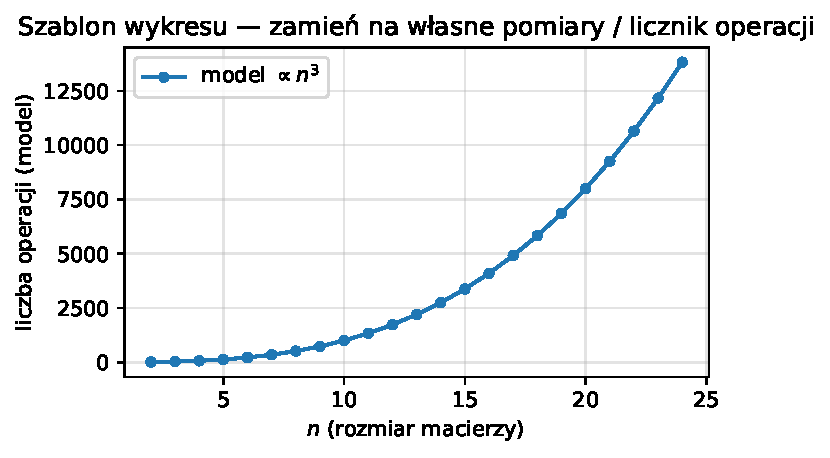
\includegraphics[width=0.72\linewidth]{szablon_flopy.pdf}
  \caption{Przykład z szablonu: model liczby operacji $\propto n^3$ w funkcji $n$ (zamień na własne pomiary).}
\end{figure}
\textit{(W zadaniach bez wykresów usuń powyższe \texttt{figure} oraz wygenerowany PDF z \texttt{figures/}.)}

\subsection{Benchmark (opcjonalnie)}
\textit{(Tu: czas vs.\ $n$, licznik operacji arytmetycznych, porównanie wariantów --- jeśli ma sens w zadaniu.)}

\section{Wnioski}
\textit{(Tu: synteza wyników, stabilność numeryczna, zgodność z teorią.)}

\end{document}
